\chapter{ Computed Torque like Controller with disturbance estimator}

Similar to the classical joint control, this controller is a completely decoupled controller, which control each joint independent and separately. In comparison to the classical joint control, which neglected all nonlinearities, this controller estimates the non linearities within the system for each joint. The controller consists of the average moment of inertia of the corresponding joint, a PD controller for the stabilization and the disturbance estimator to compensate for unknown or unmodelled system dynamics.

\begin{gather*}
\tau_{c,i} = \bar{M}_{i}\ddot{q}_{calc}+ \hat{w}(q,\dot{q})
\intertext{where:}
\begin{tabular}{>{$}l<{$} @{${}:{}$} l}
\bar{M}_{i}             & average moment of inertia of the joint         \\
\ddot{q}_{calc}        & $\ddot{q}_{D} + k_{d}\dot{e}+k_{p}e$ \\
\hat{w}(q,\dot{q}) & estimated disturbances
\end{tabular}\nonumber
\end{gather*}

For the estimation of the disturbances, a PI estimator of the following form is used:

\begin{gather*}
\hat{w}(q,\dot{q}) = l(\dot{q}_{calc} - \dot{q})
\label{eq:eq1}
\intertext{where:}
\begin{tabular}{>{$}l<{$} @{${}:{}$} l}
l & estimator parameter
\end{tabular}\nonumber
\end{gather*}

The controller structure can be seen in figure \ref{fig:ctEstimator}.
\begin{figure}[]
	\centering
	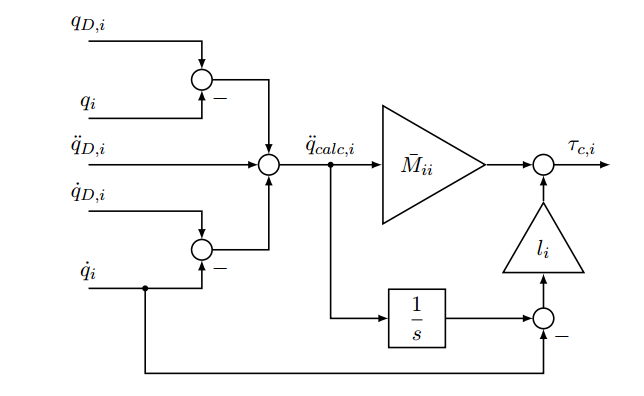
\includegraphics[width=0.55\textwidth]{pics/ctestimator.png}\\
	\caption{Controller overview of Computed Torque like controller with distortion estimator}
	\label{fig:ctEstimator}
\end{figure}

For the simulation of this controller several different parameter sets are used, which can be seen within table \ref{tab:ch5_distesti}.

\begin{table}[h]
	\begin{center}
		
		\label{tab:ch5_distesti}
		\begin{tabular}{lll}
			&                                   & According          \\
			$l_i$ & $\frac{\omega_{estim}}{\omega_n}$ & Figure             \\
			\midrule
			20    & 2                                 & \ref{fig:ch4_esti1} \\
			100   & 2                                 & \ref{fig:ch4_esti2} \\
			100   & 10                                & \ref{fig:ch4_esti3} \\
			\bottomrule
		\end{tabular}
	\caption{Controller parameters for simulations witch CT like controller with disturbance estimator}
	\end{center}
\end{table}

Figure \ref{fig:ch4_esti1} show the first simulation result. Here the controller needs around 20 seconds to settle and the initial peak of the torque is around 100Nm.\\
\begin{figure}[]
	\centering
	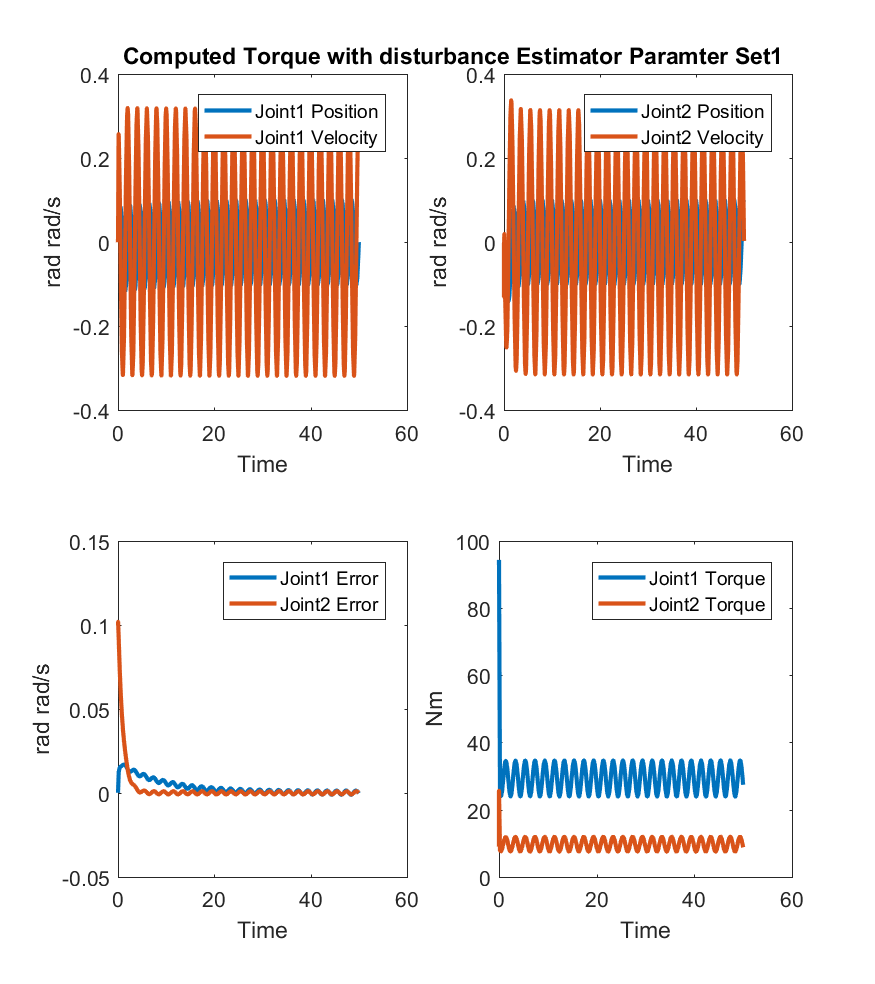
\includegraphics[width=0.85\textwidth]{pics/ComputedTorquewithdisturbanceEstimatorParamterSet1.png}\\
	\caption{CT like Controller with disturbance estimator}
	\label{fig:ch4_esti1}
\end{figure}
The next simulation uses parameters with higher gains, which lead to a settling time of around 2seconds; figure \ref{fig:ch4_esti2}. To reach the faster result a higher peak of the torque is needed.
\begin{figure}[]
	\centering
	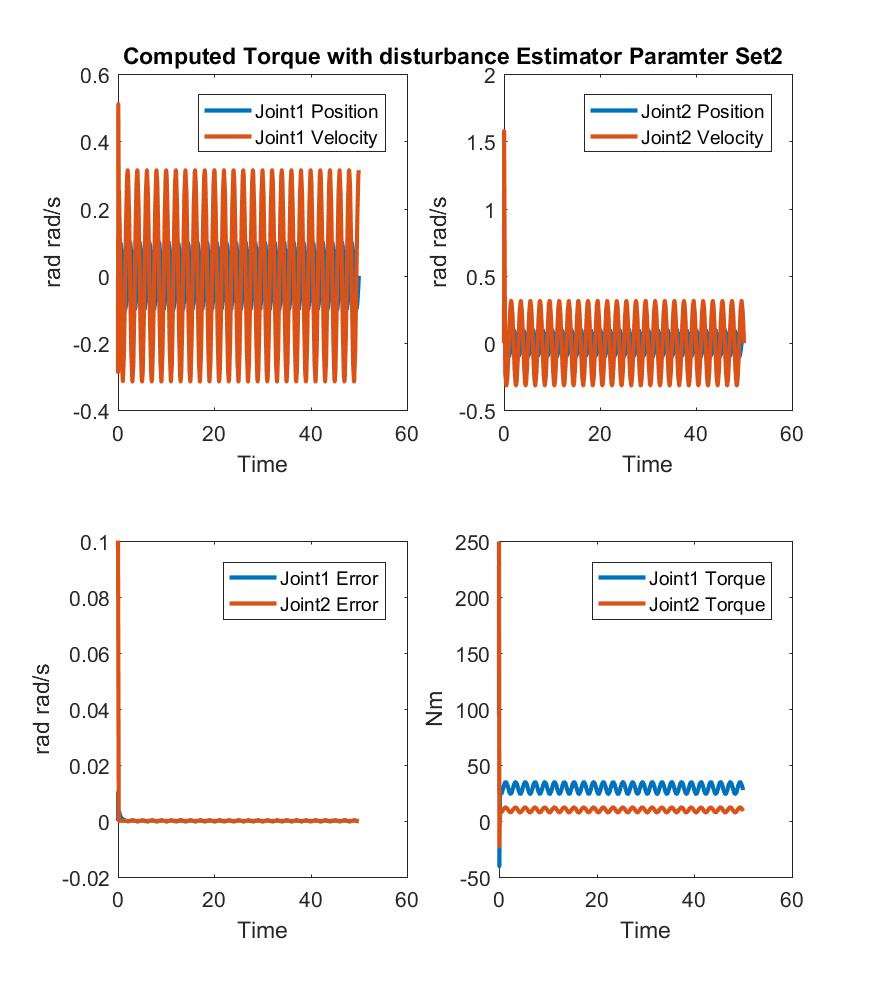
\includegraphics[width=0.85\textwidth]{pics/ComputedTorquewithdisturbanceEstimatorParamterSet2.png}\\
	\caption{CT like Controller with disturbance estimator}
	\label{fig:ch4_esti2}
\end{figure}

The last parameter set combines the advantages from the previous simulations. It has a fast settling at around 5seconds, which is short compared to the first simulation. And the torque of the system does not show similar peaks as the previous simulation with a maximum of around 100Nm.
\begin{figure}[]
	\centering
	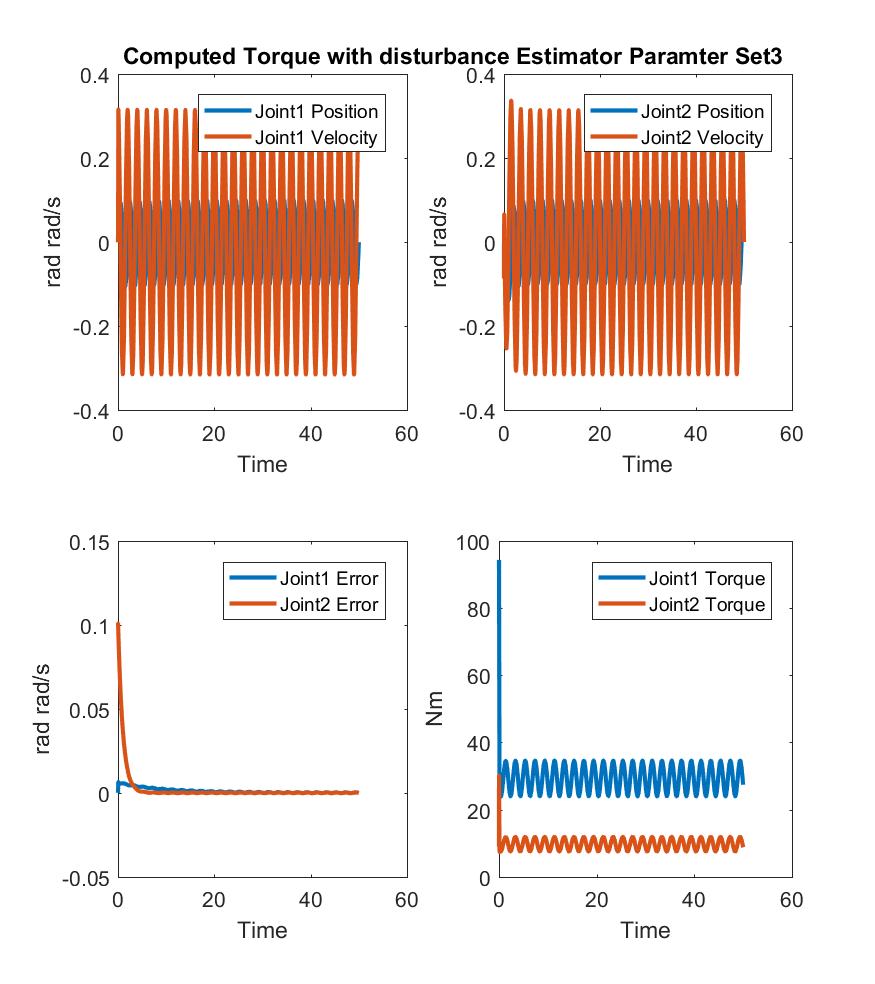
\includegraphics[width=0.85\textwidth]{pics/ComputedTorquewithdisturbanceEstimatorParamterSet3.png}\\
	\caption{CT like Controller with disturbance estimator}
	\label{fig:ch4_esti3}
\end{figure}

